\documentclass[lang=cn,11pt,a4paper,cite=authoryear]{elegantpaper}

\title{COVID-19疫情趋势预测研究}
\author{肖世莺 \and 张红丽 \and 成宏媛 \and 王瑜}
\date{}

\usepackage{array}
\newcommand{\ccr}[1]{\makecell{{\color{#1}\rule{1cm}{1cm}}}}
\usepackage{subfigure}

\begin{document}

\maketitle

\begin{abstract}
本文。。。。。。。
如果想要了解本文的相关数据和程序代码,请访问
\href{https://github.com/data-science-in-action/project-stat223}{Github::project-stat223}
。
\keywords{COVID-19,SEIR,LSTM,预测分析}
\end{abstract}

\section{引言}
COVID-19已构成全球性大流行,并已蔓延到世界上大多数国家和地区。通过了解某个地区确诊病例
的发展趋势,政府可以采取相应的政策以控制应对疫情。但是,单一的模型估计可能会得出有偏的结
果,不同数学模型产生的预测结果是不一致的。。。。。。。

\section{相关研究}

\subsection{人口增长预测模型}

[1] 沈巍,宋玉坤.人口预测方法的现状、问题与改进对策[J].统计与决策,2015(12):4-9.
人口预测方法主要分为两大类别,一种是以统计学原理为基础的传统的人口预测方法;另一种是以神经网络等智能算法为基础的创新型智能预测方法。文章对上述两类预测方法进行了比较分析,对我国目前预测方法中存在的输入数据口径不统一、不系统,文本类知识性因素被忽视以及预测模型需要发展与改进等问题进行了深入探析。

\subsection{传染病模型}

[2] 丁玲芳.几类传染病模型的定性分析
建立一类具有垂直传染的传染病模型,并得到了模型的无病平衡点和地方病平衡点的存在性及局部稳定与不稳定的充分条件。
[3] 李昊,段德光,陶学强,陈恩,高树田.传染病动力学模型及其在新型冠状病毒肺炎疫情仿真预测中的应用综述[J].医疗卫生装备,2020,41(03):7-12.
介绍了SEIR模型及元胞自动机模型、人工神经网络模型等常用的传染病动力学模型,结合新型冠状病毒肺炎疫情发展现状,总结了传染病动力学模型在疫情仿真预测中的应用情况,指出了传染病动力学模型应用的局限性。

\subsection{机器学习的数量预测应用}

[4] 陈亿雄、李苑、刘小明、李淑珍.长短记忆神经网络在流行性感冒暴发预测中的应用[J].2019
[5] 姚春晓. 基于长短时记忆神经网络的脑血管疾病预测系统研究[D].北京交通大学,2019.
[6] 黄鹏.基于机器学习的乙类传染病预测模型研究与实现[D]电子科技大学,2019
[7] Anuradha Tomar、Neeraj Gupta. Prediction for the spreed of COVID-19 in India and effectiveness of preventive measure[J]. Science of The Total Environment(2020)
[8] Bingjie Yan, Xiangyan Tang, Boyi Liu, Jun Wang, Yize Zhou, Guopeng Zheng, Qi Zou, Yao Lu, Wenxuan Tu “An Improved Method for the Fitting and Prediction of the Number of COVID-19.” arXiv preprint arXiv:2005.03446(2020)
研究表明LSTM神经网络的拟合度更接近实际值,预测精度较高。

\subsection{COVID-19的预测研究}

[9] Xiang Zhou. Forecasting the Worldwide Spread of COVID-19 based on Logistic Model and SEIR Model
结果表明,接触率,检疫规模,检疫起始时间和长度是控制流行病大小和长度的重要因素。
[10] Zifeng Yang,Zhiqi Zeng. “Modified SEIR and AI prediction of the epidemics trend of COVID-19 in China under public health interventions.” Journal of Thoracic Disease(2020)
[11] 王思远,谭瀚霖,李东杰.基于改进传染动力学易感—暴露—感染—恢复(SEIR)模型预测新型冠状病毒肺炎疫情.
[12] 卿登莉,火斌昌,杨凤. 大数据视角下遏制新型冠状病毒的举措成效分析[J].统计与管理(2020)
以上三篇都是利用SEIR模型对湖北和全国的疫情进行预测,第一篇的结论是疫情规模在2月下旬达到顶峰,到4月底逐步下降。如果将武汉封城时间推迟五天,中国大陆的疫情规模将增加三倍。第二篇预测的湖北省疫情顶点在 2月21日,5月10日左右疫情结束,累计死亡病例数为 6471例。第三篇根据有效再生数降为1的时间点可以看出湖北和全国疫情“拐点”在3月初均已出现。
[13]孙德顺,段莉,王大平,熊建义.新型冠状病毒肺炎感染的数学建模与控制策略[J].中华疾病控制杂志,2020,24(05):523-528.
选取2020年1月10到2月28日的相关数据,建立了SEIR模型结果提示对潜伏期人群和感染人群进行严格隔离,同时不断提高患者的移出率,可有效控制该传染病疫情。
[14] Zebin Zhao, Xin Li, Feng Liu, Gaofeng Zhu, Chunfeng Ma, Liangxu Wang. Prediction of the COVID-19 spread in African countries and implications for prevention and control: A case study in South Africa, Egypt, Algeria, Nigeria, Senegal and Kenya
使用最大持续(MH)参数估计方法和改进的易感性暴露传染性恢复(SEIR)模型,在南非,埃及结果表明,在南非和塞内加尔的情况下,可以通过严格控制在4月下旬基本控制该流行病。在方案二的中度控制下,感染人数将是方案一的1.43-1.55倍,疫情的控制日期将延迟约10天,阿尔及利亚,尼日利亚和肯尼亚都同意在这种情况下。在第三种控制薄弱的情况下,疫情将在5月下旬得到控制,感染病例总数将是第二种情况的两倍,埃及也符合这一预测。
[15] M.Liu, J.Ning, Y.Du, J.Cao, D.Zhang, J.Wang, M.Chen. Modelling the evolution trajectory of COVID-19 in Wuhan, China: experience and suggestions
结果表明,该四阶段SEIR模型可有效地捕获了COVID-19的演变轨迹,有效预测COVID-19的峰值,大小和持续时间。由于英国在COVID-19的初期反应不正确,因此它将成为另一个震中。
[16] Yamini Marimuthu, Bharathnag Nagappa, Nandini Sharma, Saurav Basu, Kamal Kishore Chopra.COVID-19 and tuberculosis: A mathematical model based forecasting in Delhi, India
研究发现公共卫生干预措施的实施将延迟高峰期并导致流行曲线趋于平坦。在没有公共卫生干预措施的情况下,高峰期将在第94天出现。如果存在有效的干预措施,例如锁定42天,社交距离,接触者追踪和案例隔离,则高峰期将延迟44天,并在第138天发生。
[17] Novanto Yudistira .“COVID-19 growth prediction using multivariate long short term memory.” arXiv preprint arXiv :2005.04809v1(2020)
Novanto Yudistira(2020)使用长期短期记忆(LSTM)方法来了解covid-19随时间增长的相关性。发现随着时间的推移很难获得完全相同数量的确诊病例,但是LSTM能够在实际和预测之间提供相似的模式。结果表明,LSTM是一种有前途的预测工具通过从大数据中学习并潜在地传播covid-19大流行能够预测未来的爆发。
[18] Vinay Kumar Reddy Chimmula, Lei Zhang, Time Series Forecasting of COVID-19 transmission in Canada Using LSTM Networks, Chaos, Solitons and Fractals (2020) doi: https://doi.org/10.1016/j.chaos.2020.109864
Vinay Kumar Reddy Chimmula, Lei Zhang(2020)根据约翰·霍普金斯大学和加拿大卫生部门提供的公共数据集基于截至2020年3月31日的可用数据。评估了关键特征,以预测加拿大和全球当前COVID-19爆发的趋势和可能的停止时间。在本文中,使用长期短期记忆(LSTM)网络,结果显示爆发的可能终点是2020年6月左右。此外,我们还比较了加拿大,意大利和美国的传播率,美国的传播率最高,加拿大的传播率最低。

\section{研究方法}

\subsection{SEIR模型}
SEIR模型将研究对象分为S、E、I、R4种类型;1)$S$为易感状态(susceptible),表示潜在的可
感染人群,个体在感染之前是处于易感状态的,即该个体有可能被邻居个体感染。2)$E$为潜伏状态
(exposed),表示已经被感染但没有表现出感染症状来的群体。3)$I$为感染状态(infected),
表示表现出感染症状的人,该个体还会以一定的概率感染其能接触到的易感个体。4)$R$为移出状态
(removed),表示脱离系统不再受到传染病影响的人。

记$S(t)$、$E(t)$、$I(t)$、$R(t)$分别为时刻$t$的易感人群数、潜伏人群数、感染人群数、移出
人群数,显然有$S(t)+E(t)+I(t)+R(t)=N$,其中$N$为种群的个体数。

假设一个易感状态在单位时间$\tau$里与感染个体接触并被传染的概率为$\beta$。由于易感个体的
比例为$S/N$,时刻$t$网络中总共有$I(t)$个感染个体,所以易感个体的数目按照如下变化率变化:
\begin{equation}
\frac{dS}{dt}=-\frac{\beta SI}{N}
\end{equation}
相应地,潜伏个体的数目按照如下变化率增加,并且整体以单位时间概率$\sigma$转化为感染个体:
\begin{equation}
\frac{dE}{dt}=\frac{\beta SI}{N}-\sigma E
\end{equation}
感染个体数目由潜伏群体提供,个体同时以单位时间概率$\gamma$转化为移除状态:
\begin{equation}
\frac{dI}{dt}=\sigma E-\gamma I
\end{equation}
相应地移除个体以概率$\gamma$由感染群体往移除个体转化:
\begin{equation}
\frac{dR}{dt}=\gamma I
\end{equation}
\subsection{LSTM模型}
LSTM模型(Long Short-Term Memory)是一种用于深度学习领域的递归神经网络(RNN)架构在传统
的RNN模型中,所使用的训练算法是时序反向传播算法(Back Propagation Trough 
Time,即BPTT)。循环网络的目的是能够对输入的序列进行准确的分类,这主要靠误差值(预测结果
与真实结果的差距)的反向传播和梯度下降来实现。反向传播从最后的误差值开始,将误差值以某种
形式,经过每个隐藏层向输入层逐层反向传播,按照一定的比例将误差分摊给所有的单元,从而获得
各层单元的误差信号,以此作为修正各个单元权值的依据。反向传播算法的目的就是寻找能够最大限
度地减小误差的权重。最小化误差的实质是一个优化问题,这就需要计算误差对权重的偏导,将偏导
数运用到梯度下降算法中,以调整权重减少误差。而BPTT是循环网络依赖于反向传播的一种扩展,通
过一系列定义明确、有序的计算来表达时间,这些计算将一个时间步与下一个时间步联系起来。当模
型运算时间较长时,需要回传的残差会呈现指数下降,导致网络权重更新缓慢,使RNN模型的长期记
忆效果无法得以体现,因此LSTM模型应运而生。LSTM模型由\cite{hochreiter1997lstm}提出,在
各隐藏层的神经元单元之间增加了记忆单元,可以学习长期依赖信息,避免了RNN无法解决的长期依
赖问题。此后许多学者对其进行了改进,使得LSTM在许多问题上得到了广泛的使用,并取得相当巨大
的成功\citep{gers2000learning, graves2005bidirectional, graves2005framewise, 
schmidhuber2007training, bayer2009evolving, schaul2010pybrain, 
graves2013hybrid, bayer2014Learning}。

\begin{figure}[htp]
	\centering
	\subfigure[RNN] {
		\begin{minipage}{0.48\linewidth}
			\centering
			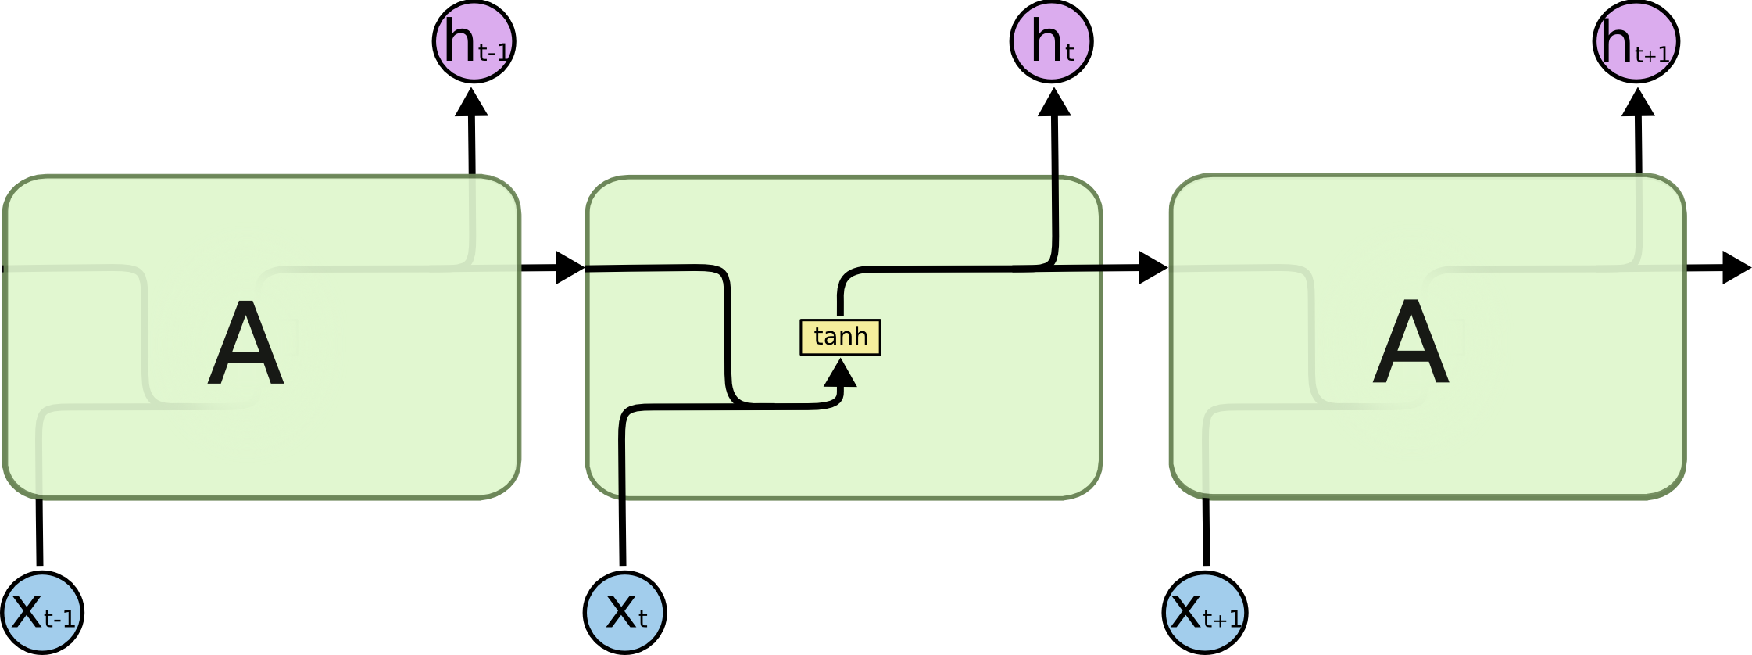
\includegraphics[width=7.0cm]{RNN.pdf}
		\end{minipage}
	}
	\subfigure[LSTM] {
		\begin{minipage}{0.48\linewidth}
			\centering
			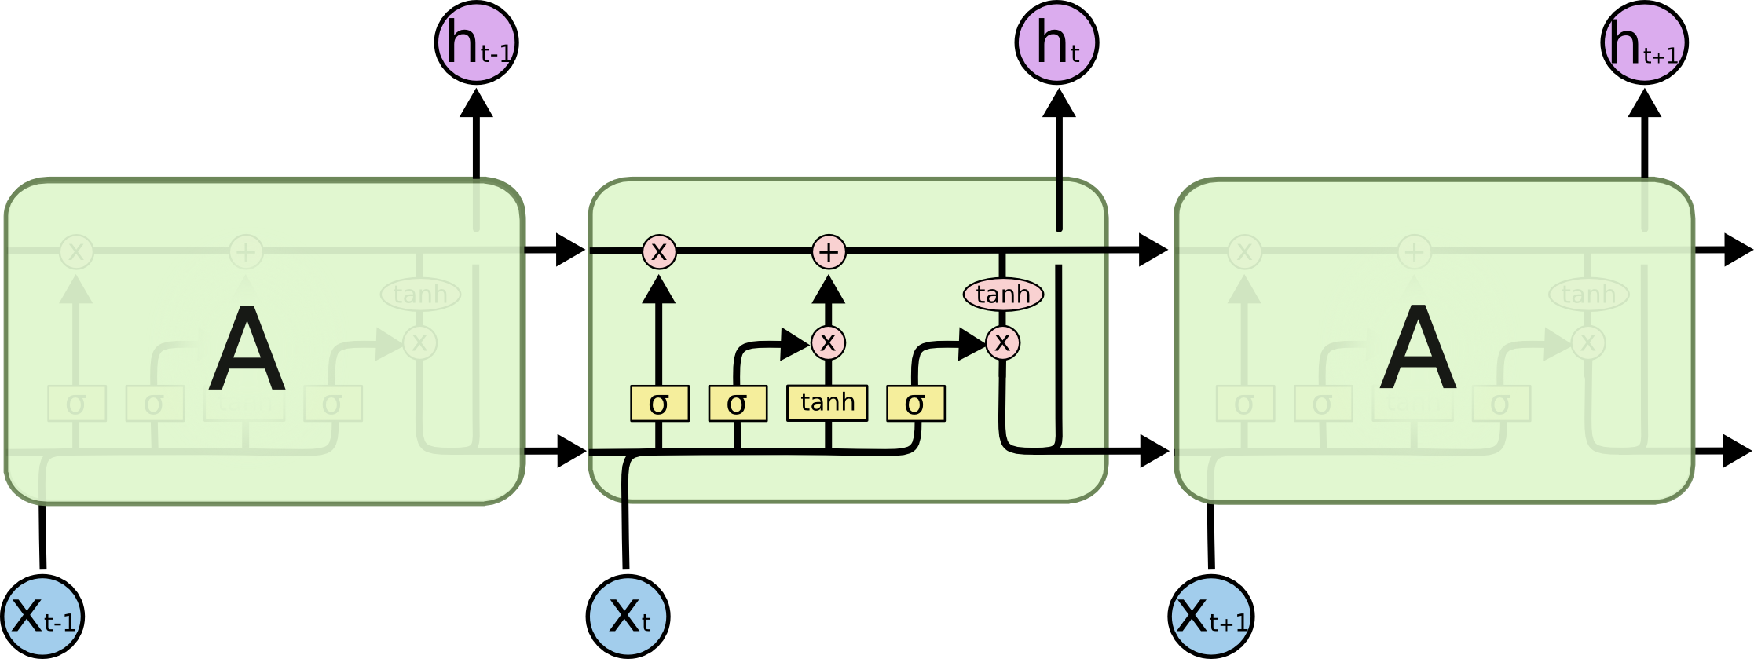
\includegraphics[width=7.0cm]{LSTM.pdf}
		\end{minipage}
	}
    \caption{RNN模型和LSTM模型的结构}
	\label{fig:structure}
\end{figure}

图\ref{fig:structure}显示了RNN模型与LSTM模型的结构,其中蓝色圆圈$x_t$表示输入信息,紫
色圆圈$h_t$表示输出信息,黄色框表示神经网络层,粉色圆圈表示逐点运算,例如矢量加法。每条
线上都承载着从一个节点的输出到另一个节点的输入的矢量。合并的线表示向量的连接,而分开的线
表示其内容被复制,然后分配到不同的位置。由图\ref{fig:structure}可见,RNN与LSTM最大的
区别在于——LSTM中最顶层多了一条信息传送带,即细胞状态$C_t$,也就是信息记忆的地方,这也是LSTM
的核心。

LSTM通过称作门(gate)的结构调节,具有删除或添加信息到细胞状态的能力。门是一种选择性地让
信息通过的方式,由$\sigma$(sigmoid)神经网络层和逐点乘法运算组成。$\sigma$层输出$0$
到$1$之间的数值,描述每个信息量可以通过多少。$0$代表“不许任何量通过”,$1$代表“允许任意
量通过”。常见的LSTM单元由一个细胞、一个输入门(input gate)、一个输出门(output gate)
和一个遗忘门(forget gate)组成。细胞会记住任意时间间隔内的值,并且三个门控制着进出单元
的信息流。

LSTM模型中,第一步是决定从细胞状态中丢弃哪些信息。这个决定通过一个称为“遗忘门层”的$\sigma$
层决定。该门会读取$h_{t-1}$和$x_t$作为输入,为细胞状态$C_t$中的每个数输出一个在$0$到$1$
之间的数值,记为$f_t$,表示保留多少信息,$1$表示“完全保留信息”,$0$表示“完全舍弃信息”。
\begin{equation}
f_t=\sigma(W_{f} \cdot [h_{t-1},x_{t}]+b_{f})
\end{equation}

第二步是在细胞状态中存储哪些信息。首先是由称为“输入门层”的$\sigma$层决定哪些信息需要更
新,该概率表示为$i_t$;然后输入门层中的tanh层创建一个新的候选值向量$\tilde{C_t}$,将其
增加到细胞状态中。
\begin{gather}
i_t=\sigma(W_{i} \cdot [h_{t-1},x_{t}]+b_i) \\
\tilde{C_t}={\rm tanh}(W_{C} \cdot [h_{t-1},x_{t}]+b_C)
\end{gather}

第三步是更新旧的细胞状态。$f_t$表示忘记上一次信息$C_t$的程度,$i_t$表示将候选值$\tilde{C_t}$
加入的程度,通过对第二步中两个信息的结合,真正实现了移除哪些旧的信息,增加哪些新信息,最
后得到了本细胞的状态$C_t$。
\begin{equation}
C_t=f_t*C_{t-1}+i_t*\tilde{C_t}
\end{equation}

最后是确定要输出的内容,即决定作出什么样的预测。首先,通过运行称为“输出门层”的$\sigma$
层来决定输出细胞状态$C_t$的哪些部分;然后,将细胞状态通过tanh层进行处理,使值在$-1$与$1$
之间,然后与$\sigma$层的输出相乘,最终输出决定输出的那部分。
\begin{gather}
o_t=\sigma(W_o \cdot [h_{t-1},x_t]+b_o) \\
h_t=o_t*{\rm tanh}(C_t)
\end{gather}

\begin{figure}[htp]
	\centering
	\subfigure[遗忘门:舍弃信息] {
		\begin{minipage}{0.48\linewidth}
			\centering
			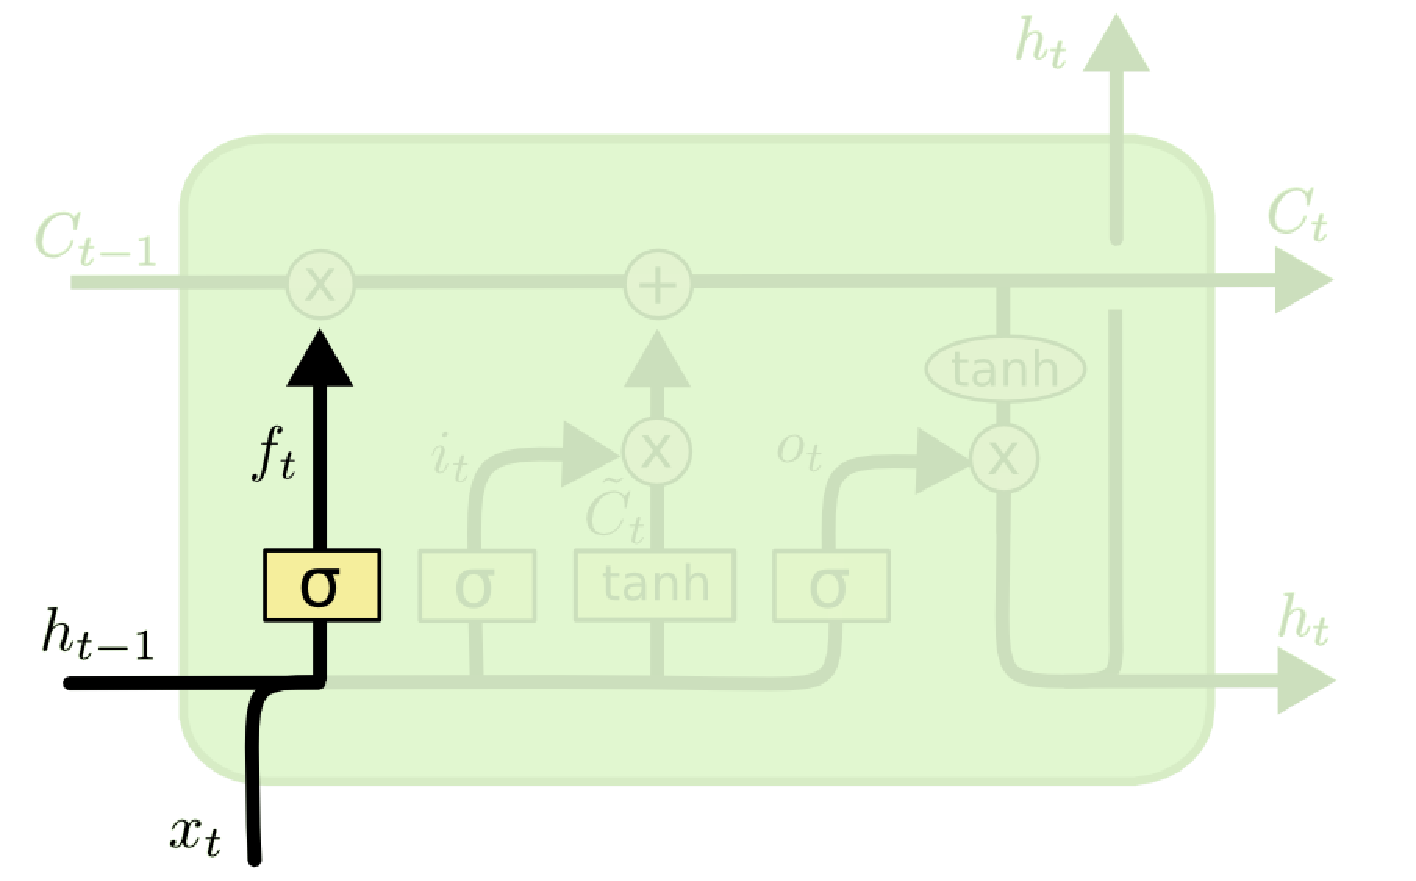
\includegraphics[width=7.0cm]{forget.pdf}
		\end{minipage}
	}
    \subfigure[输入门:存储信息] {
		\begin{minipage}{0.48\linewidth}
			\centering
			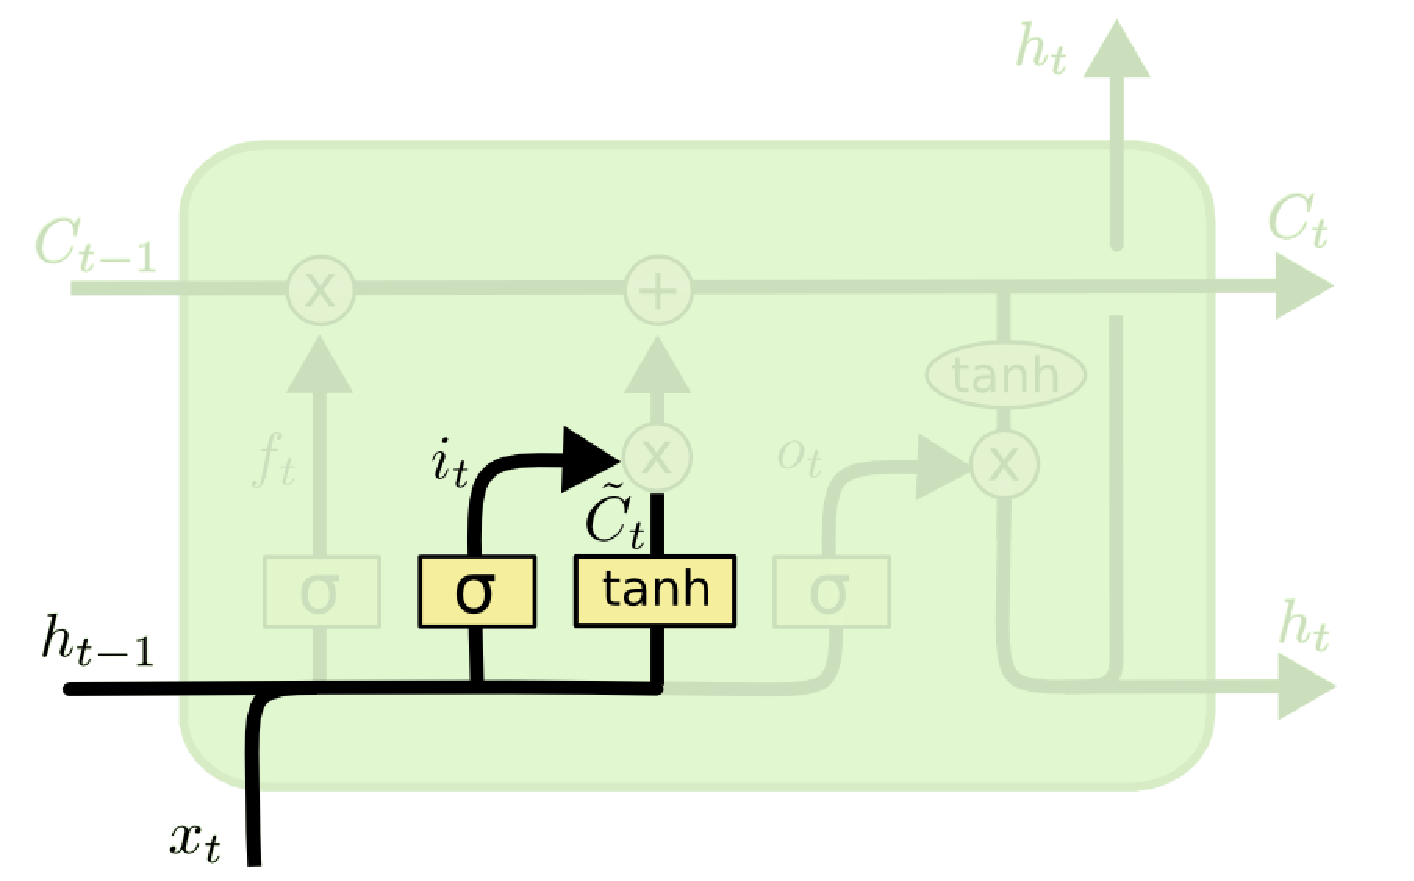
\includegraphics[width=7.0cm]{input.pdf}
		\end{minipage}
	}
	\\
	\subfigure[更新细胞状态] {
		\begin{minipage}{0.48\linewidth}
			\centering
			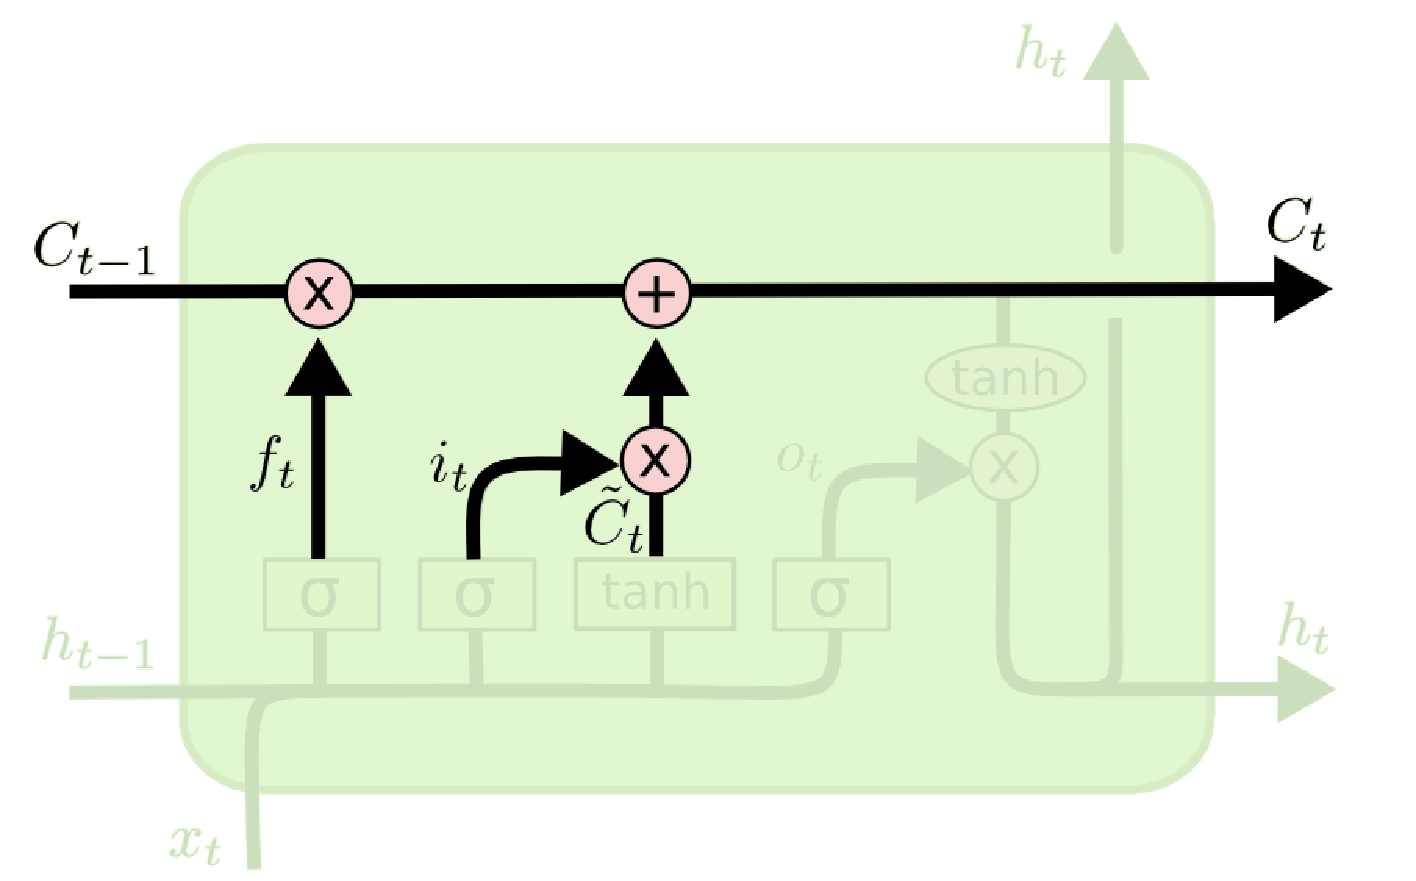
\includegraphics[width=7.0cm]{update.pdf}
		\end{minipage}
	}
	\subfigure[输出门:输出] {
		\begin{minipage}{0.48\linewidth}
			\centering
			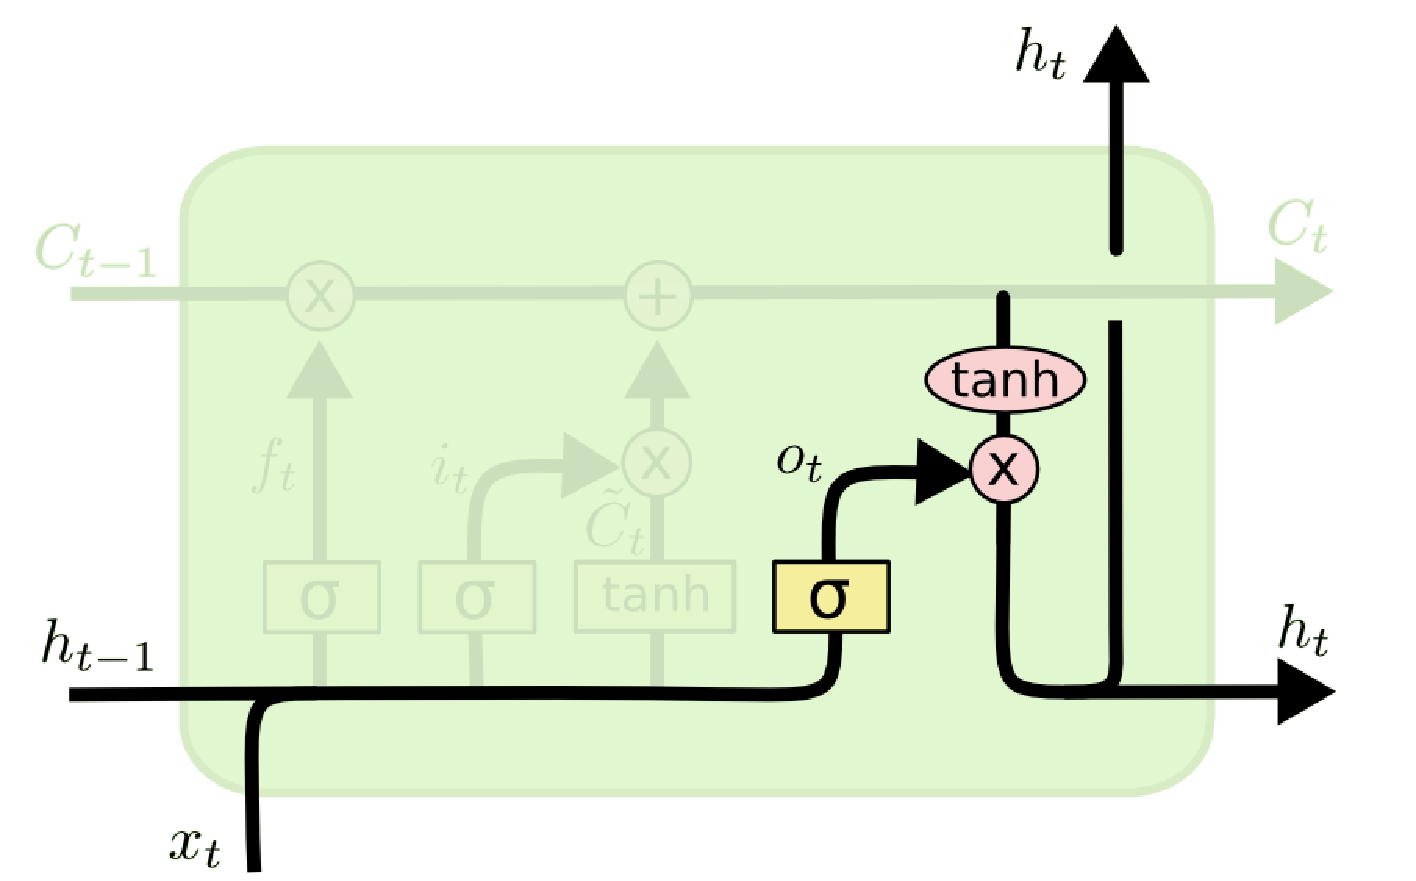
\includegraphics[width=7.0cm]{output.pdf}
		\end{minipage}
	}
    \caption{LSTM信息的流动}
	\label{fig:LSTM}
\end{figure}

\section{疫情发展现状}

我们选取了全球除中国外,疫情状况最为严重的八个国家作为研究对象,以八个国家为代表来对全球疫情数据有一个大概的分析处理
首先对八个国家累计确诊人数绘制折线图,来对各国疫情爆发所处阶段有一个大致了解。在绘制八国疫情图是,起始日期是不同的,选取各国累计确诊数超过100例那天为起始日期,如意大利起始日期设定为2020那2月23日。   
从图一可以看出,美国确诊人数增长速度是远高于其余七个国家, 在美国如此迅猛的增势对比下七国的确诊人数增长较为平缓,下面将美国从折线图中暂时去掉来对剩余的七个国家的疫情发展现状进行展示。

一般来说疫情曲线遵循上升达到顶峰最后下降这一趋势。由上图可以看出,七个国家中巴西和俄罗斯上升速度比较明显,且巴西的增长速度要明显高于俄罗斯,剩余的五个国家上升趋势依然存在,但逐渐趋于平缓,但七个国家的均未到达其拐点及顶峰位置。由目前来看,对疫情的防控措施不容放松,各国要坚持贯彻疫情相关管理政策及落实各种防疫措施。
进一步建立已请相关指标对各国疫情数据有进一步的了解
	累计确诊	死亡率	治愈率	占比
Brazil	438812	5.0%	23.6%	0.0022 
France	186238	9.7%	19.6%	0.0028 
Germany	182452	2.3%	42.9%	0.0022 
Italy	231732	10.4%	23.5%	0.0038 
Russia	379051	0.8%	10.4%	0.0026 
Spain	284986	8.5%	32.6%	0.0061 
United Kingdom	269127	11.1%	1.3%	0.0040 
US	1768461	4.5%	7.9%	0.0054 

截止5月24日,美国确诊人数已经超过了176万。累计确诊人数不仅是这八个国家中最多的,也是全球最多的。通过死亡率来看,俄罗斯死亡率是最低的,不足1\%,英国死亡率高达 11.1\% ,是八个国家中死亡最为严重的国家,对应英国治愈率也是八个国家中最低的,这个结果是由其医疗系统的匮乏造成的,医疗的不到位使英国对与患者的收治能力较低,病人只有在症状较为严重,较为危急时才能得以入院治疗,对于病情严重的患者,死亡率很高和治愈率很低也就不难理解了。德国治愈率是最高的,这跟德国工业体系的完善有很大关系,对于口罩、防护服呼吸机等这类防疫设备能做到自主生产,最大程度满足了德国人民的需要。而且德国在疫情爆发后,也做到了严格防控,充分隔离。除德国外,巴西和意大利的治愈率也处在了一个相对较高的水平(23\%左右)。上表中的占比是指该国累计确诊人数占该国总人口数的比重,可以看出西班牙确诊人数占比是最多的,其次就是美国了。

\section{实证分析}

\subsection{SEIR模型}
在进行seir模型预测的时候我们使用到了死亡率,治愈率,国家总人口,现有确诊,死亡率治愈率计算时使用数据均来源于约翰霍普金斯大学的官网疫情数据。
$死亡率=(∑_i^n▒每日累计死亡人数/每日累计确诊人数)/n$
$治愈率=(∑_i^n▒每日累计治愈人数/每日累计确诊人数)/n$
其中n为研究天数
基于SEIR模型,文章预测了八个国家的疫情发展趋势,表1详细地列出了八个国家的预测结果和增长轨迹。

接下来展示各个国家SEIR模型结果,曲线从上到下依次是国家总人口、易感人数、潜伏期人数、感染人数以及移除人数。初始阶段全国总人数是等于易感人数的,但随着疫情的传播,,易感人数在下降,同时由于死亡人数的增加国家总人口数也有所下降。最终在彼此作用下国家疫情发展会达到动态平衡的状态。
	Brazil	France	Germany	Italy	Russia	Spain	UK	US
Days to Peak	81	80	169	85	51	130	49	55
Peak value(*104 active)	2261.3	744.5	104.3	499.5	6290	117.5	2965.8	13643

从图中可以看出法国在疫情发生后易感人数会有一个大幅下降,也就是说,潜伏期人数的增加幅度比较大,感染人数和易感人数交叉时感染人数会达到一个顶峰。模型预测,法国会在初始日期80天后达到这个顶峰,也就是月日累计确诊人数达到顶峰,预测峰值为744.5万人。
相较于法国,德国易感人数下降的幅度较少,感染人数和易感人数并未有交叉,模型预测德国在169天累计确诊人数达到峰值,时间处在一个比较长的跨度,表面德国疫情扩散还是处在一个比较慢的状态,且预测峰值人数也是八个国家中最少的,预测峰值人数为104.33万人。

不同于别的国家,英国的SEIR曲线,易感人数和全国总人口在预测期间急速下降,最终停在了一个很低的水平,表明应该的疫情扩散极其迅速以及蔓延的后果(参照其死亡率及治愈率)特别严重。截至目前英国累计确诊人数增长还是处在一个上升的状态,如果应该政府不采取更加严格的措施的话,模型预测结果是很有可能成为现实。模型预测英国的峰值日期来临时间很短,将其设定在了初始日期后的49天,并预测最终累计确诊人数会超过一亿三千万人。这个预测结果需要政府得到重视。
图为西班牙的SEIR模型仿真结果,西班牙有着较高的治愈率,潜伏状态和感染状态的人数都在疫情发生一百多天以后才开始加速增长,在第125天~第130天达到峰值,之后开始下降。从图上也可以很明显地看出在疫情结束后,西班牙的累计确诊人数相对较少。模型预测峰值时累计确诊人数为117万人。

从美国的SEIR模型图中可以看出美国峰值感染人数处在一个极高的水平,在模型达到稳定后,国家总人口与移除人数处在了非常接近的高度,这表明,照目前美国传播速度,在疫情发展后期,美国大部分公民都将感染新型冠状病毒,易感人数数量极低,模型将峰值日期设定在了初始日期后的55天,并预测最终累计确诊人数会超过一亿三千万人。这个结果是八个国家中预测的累计确诊人数最多的。
图为俄罗斯的SEIR模型仿真结果,由于俄罗斯治愈率相对较低,在疫情发生后的第25天~第35天潜伏状态和感染状态的人数就开始加速增长,在第41天~51天达到高峰,随后开始下降。模型预测俄罗斯的现有感染人数峰值在500万以上,相对较高。而图中也可以发现,在疫情结束后,俄罗斯累计确诊人数占全国总人数的比例也相对较高。

图为意大利的SEIR模型仿真结果,可以看出在疫情发展初期潜伏状态和感染状态的在都处于上升趋势,在第30天~第40天左右开始加速增长,在第75天~第85天达到高峰,之后开始下降直至消失。而在疫情结束后累计确诊人数达到499万人。
图中可以看出巴西与意大利的SEIR结果比较类似,但不同的是,模型将巴西的峰值日期设立在了起始日期后的70~81天,较意大利峰值来临较早一点,但峰值累计确诊人数却远大于意大利,模型预测峰值时累计确诊人数会达2261.3万人,疫情扩张的结果也相当严重。


\subsection{LSTM模型}

\section{讨论}

\bibliography{report}

\end{document}
